\documentclass{scrartcl}
\usepackage{pgfplots}
\usepackage{graphicx}
\usepackage[left=1cm, right=1cm, top=1cm, bottom=3cm]{geometry}

\renewcommand{\thesection}{\Roman{section}}

\usepackage{titlesec}
\titlelabel{\thetitle)\quad}

% given
\begin{document}

	\title{\vspace{-2cm}Compte-rendu de travaux pratiques de physique}
	\subtitle{Analyse informatique d'enregistrements vidéos}
	\author{Benjamin Loison (MPSI 1)}
	\date{23 février 2019}
	\maketitle

  \setcounter{section}{1}
	\section{Exemples élémentaires}

		\subsection{Chute libre}
		
			\subsubsection{BallDrop}

			\begin{tikzpicture}
			\begin{axis}[
				xlabel=$t$ (en s),
				ylabel=$y(t)$ (en m)]
			\addplot[color = red, mark = x] coordinates {
				(0, 0.4886)
				(0.03333, 0.5672)
				(0.06667, 0.6388)
				(0.1, 0.6963)
				(0.1333, 0.7434)
				(0.1667, 0.7764)
				(0.2, 0.8059)
				(0.2333, 0.8196)
				(0.2667, 0.8245)
				(0.3, 0.8207)
				(0.3333, 0.8045)
				(0.3667, 0.7831)
				(0.4, 0.746)
				(0.4333, 0.7)
				(0.4667, 0.6418)
				(0.5, 0.5765)
				(0.5333, 0.4955)
				(0.5667, 0.4074)
				(0.6, 0.3088)
				(0.6333, 0.1962)
				(0.6667, 0.07132)
				(0.7, -0.06061)
			};
			\end{axis}
		\end{tikzpicture}
		
		\noindent On a: $y(T) = y_{max} - \frac{gT^2}{2}$ avec $T = t - t_{ymax}$.\\
		Donc: $g = \frac{2 * (y_{max} - y(T_{fin}))}{T_{fin}^2}$
		On a alors: $g = \frac{2 * (0.8245 - (-0.0606))}{(0.7 - 0.2667)^2} = 9.43$ $m.s^{-2}$
		
		\subsubsection{BallTossUp}
		
			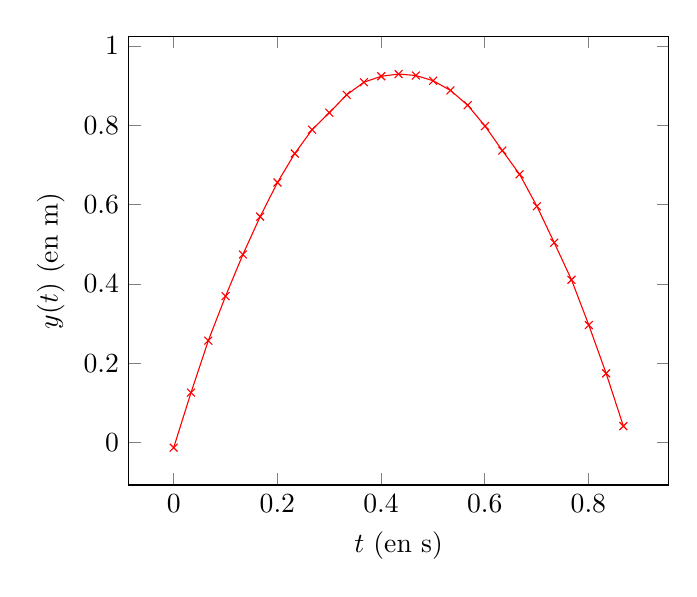
\begin{tikzpicture}
			\begin{axis}[
				xlabel=$t$ (en s),
				ylabel=$y(t)$ (en m)]
			\addplot[color = red, mark = x] coordinates {
				(0, -0.01311)
				(0.03337, 0.1255)
				(0.06673, 0.2566)
				(0.1001, 0.3689)
				(0.1335, 0.4738)
				(0.1668, 0.5693)
				(0.2002, 0.6554)
				(0.2336, 0.7285)
				(0.2669, 0.7884)
				(0.3003, 0.8315)
				(0.3337, 0.8764)
				(0.367, 0.9082)
				(0.4004, 0.9232)
				(0.4338, 0.9288)
				(0.4671, 0.9251)
				(0.5005, 0.912)
				(0.5339, 0.8876)
				(0.5672, 0.8502)
				(0.6006, 0.7977)
				(0.634, 0.7359)
				(0.6673, 0.676)
				(0.7007, 0.5955)
				(0.7341, 0.5037)
				(0.7674, 0.4101)
				(0.8008, 0.2959)
				(0.8342, 0.1742)
				(0.8675, 0.0412)
			};
			\end{axis}
		\end{tikzpicture}		
		
		De même on a: $g = \frac{2 * (y_{max} - y(T_{fin}))}{T_{fin}^2}$
		On a alors: $g = \frac{2 * (0.9288 - 0.0412)}{(0.8675 - 0.4338)^2} = 9.44$ $m.s^{-2}$

		\subsection{Pendule pesant}
			
			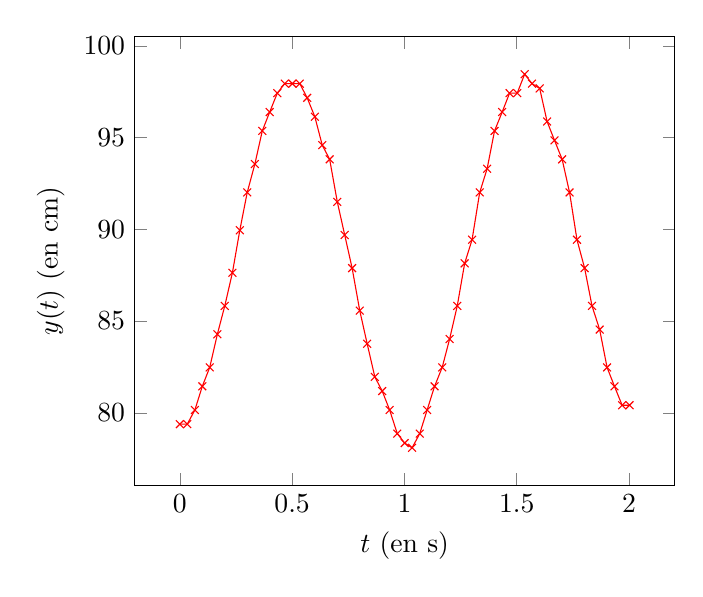
\begin{tikzpicture}
			\begin{axis}[
				xlabel=$t$ (en s),
				ylabel=$y(t)$ (en cm)]
			\addplot[color = red, mark = x] coordinates {
				(0, 79.381)
				(0.033, 79.381)
				(0.067, 80.154)
				(0.1, 81.443)
				(0.133, 82.474)
				(0.167, 84.278)
				(0.2, 85.824)
				(0.234, 87.629)
				(0.267, 89.948)
				(0.3, 92.01)
				(0.334, 93.556)
				(0.367, 95.361)
				(0.4, 96.391)
				(0.434, 97.422)
				(0.467, 97.938)
				(0.501, 97.938)
				(0.534, 97.938)
				(0.567, 97.165)
				(0.601, 96.134)
				(0.634, 94.587)
				(0.667, 93.814)
				(0.701, 91.495)
				(0.734, 89.69)
				(0.767, 87.886)
				(0.801, 85.567)
				(0.834, 83.763)
				(0.868, 81.958)
				(0.901, 81.185)
				(0.934, 80.154)
				(0.968, 78.866)
				(1.001, 78.35)
				(1.034, 78.093)
				(1.068, 78.866)
				(1.101, 80.154)
				(1.134, 81.443)
				(1.168, 82.474)
				(1.201, 84.02)
				(1.235, 85.824)
				(1.268, 88.144)
				(1.301, 89.433)
				(1.335, 92.01)
				(1.368, 93.299)
				(1.401, 95.361)
				(1.435, 96.391)
				(1.468, 97.422)
				(1.502, 97.422)
				(1.535, 98.453)
				(1.568, 97.938)
				(1.602, 97.68)
				(1.635, 95.876)
				(1.668, 94.845)
				(1.702, 93.814)
				(1.735, 92.01)
				(1.768, 89.433)
				(1.802, 87.886)
				(1.835, 85.824)
				(1.869, 84.536)
				(1.902, 82.474)
				(1.935, 81.443)
				(1.969, 80.412)
				(2.002, 80.412)
			};
			\end{axis}
		\end{tikzpicture}\\\\\\		
			
			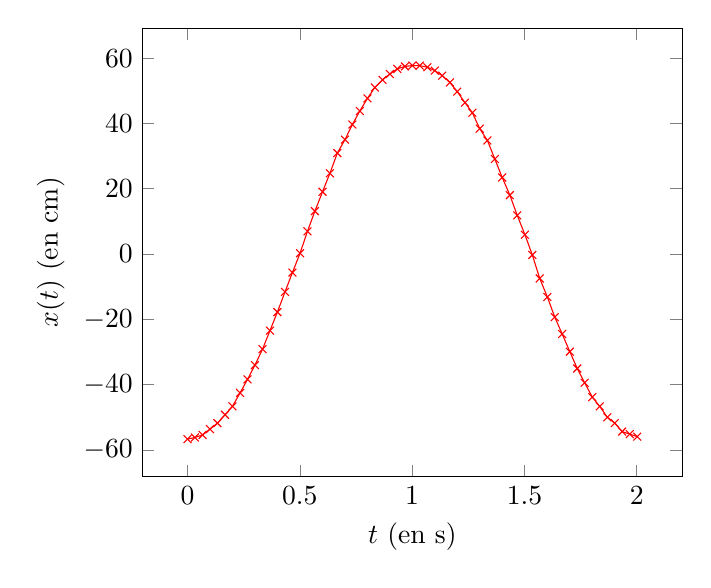
\begin{tikzpicture}
			\begin{axis}[
				xlabel=$t$ (en s),
				ylabel=$x(t)$ (en cm)]
			\addplot[color = red, mark = x] coordinates {
				(0, -56.701)
				(0.033, -56.185)
				(0.067, -55.412)
				(0.1, -53.608)
				(0.133, -51.804)
				(0.167, -49.227)
				(0.2, -46.649)
				(0.234, -42.526)
				(0.267, -38.402)
				(0.3, -34.021)
				(0.334, -29.124)
				(0.367, -23.454)
				(0.4, -17.783)
				(0.434, -11.598)
				(0.467, -5.67)
				(0.501, 0.258)
				(0.534, 6.959)
				(0.567, 13.144)
				(0.601, 19.072)
				(0.634, 24.742)
				(0.667, 30.928)
				(0.701, 35.051)
				(0.734, 39.691)
				(0.767, 43.814)
				(0.801, 47.68)
				(0.834, 51.031)
				(0.868, 53.35)
				(0.901, 55.154)
				(0.934, 56.701)
				(0.968, 57.474)
				(1.001, 57.732)
				(1.034, 57.732)
				(1.068, 57.216)
				(1.101, 56.185)
				(1.134, 54.639)
				(1.168, 52.577)
				(1.201, 49.742)
				(1.235, 46.392)
				(1.268, 43.299)
				(1.301, 38.402)
				(1.335, 34.794)
				(1.368, 29.124)
				(1.401, 23.454)
				(1.435, 18.041)
				(1.468, 11.856)
				(1.502, 5.928)
				(1.535, -0.258)
				(1.568, -7.474)
				(1.602, -13.144)
				(1.635, -19.33)
				(1.668, -24.484)
				(1.702, -29.897)
				(1.735, -35.051)
				(1.768, -39.433)
				(1.802, -43.814)
				(1.835, -46.649)
				(1.869, -50)
				(1.902, -51.804)
				(1.935, -54.381)
				(1.969, -55.154)
				(2.002, -55.928)
			};
			\end{axis}
		\end{tikzpicture}\\\\\\
					
					
			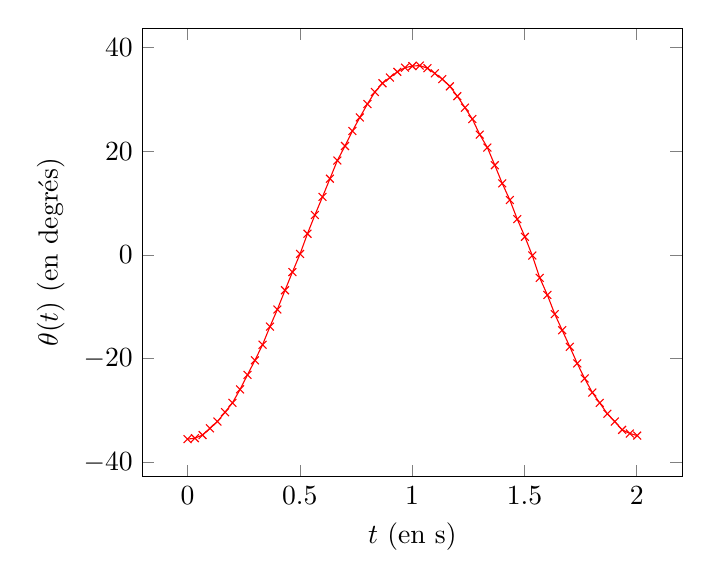
\begin{tikzpicture}
			\begin{axis}[
				xlabel=$t$ (en s),
				ylabel=$\theta(t)$ (en degrés)]
			\addplot[color = red, mark = x] coordinates {
				(0, -35.5)
				(0.033, -35.3)
				(0.067, -34.7)
				(0.1, -33.4)
				(0.133, -32.1)
				(0.167, -30.3)
				(0.2, -28.5)
				(0.234, -25.9)
				(0.267, -23.1)
				(0.3, -20.3)
				(0.334, -17.3)
				(0.367, -13.8)
				(0.4, -10.5)
				(0.434, -6.8)
				(0.467, -3.3)
				(0.501, 0.2)
				(0.534, 4.1)
				(0.567, 7.7)
				(0.601, 11.2)
				(0.634, 14.7)
				(0.667, 18.2)
				(0.701, 21)
				(0.734, 23.9)
				(0.767, 26.5)
				(0.801, 29.1)
				(0.834, 31.4)
				(0.868, 33.1)
				(0.901, 34.2)
				(0.934, 35.3)
				(0.968, 36.1)
				(1.001, 36.4)
				(1.034, 36.5)
				(1.068, 36)
				(1.101, 35)
				(1.134, 33.9)
				(1.168, 32.5)
				(1.201, 30.6)
				(1.235, 28.4)
				(1.268, 26.2)
				(1.301, 23.2)
				(1.335, 20.7)
				(1.368, 17.3)
				(1.401, 13.8)
				(1.435, 10.6)
				(1.468, 6.9)
				(1.502, 3.5)
				(1.535, -0.1)
				(1.568, -4.4)
				(1.602, -7.7)
				(1.635, -11.4)
				(1.668, -14.5)
				(1.702, -17.7)
				(1.735, -20.9)
				(1.768, -23.8)
				(1.802, -26.5)
				(1.835, -28.5)
				(1.869, -30.6)
				(1.902, -32.1)
				(1.935, -33.7)
				(1.969, -34.4)
				(2.002, -34.8)
			};
			\end{axis}
		\end{tikzpicture}
				
			\noindent Oui $\theta(t)$ est une fonction sinusoïdale de période $T$ = 2.00 secondes. Ce qui est proche de la valeur théorique: $T = 2\pi\sqrt{\frac{l}{g}} = 2\pi\sqrt{\frac{1}{9.807}}$ = 2.006 s.\\
			On obtient alors le portait de phase suivant:
			
			\begin{figure}[ht!]
				\centering
				\includegraphics[width=90mm]{"portrait de phase".jpg}
				\caption{Portrait de phase}
			\end{figure}
			
		\subsection{Faster than gravity}
		
			\subsubsection{Premier essai}
			
				Cette expérience a comme caractéristique que le centre de masse de la barre, situé vers le centre de celle-ci, tombe a une accélération de $g$ tandis que entraîné le bout de la barre parcourt pendant la même durée de chute une distance plus grande donc tombe avec une accélération supérieure à $g$.\\
				L'utilité de la balle de golf est ici puisqu'elle chute avec une accélération $g$ de la voir se décoller puis retomber dans le réceptacle en aval.
				On calcule la valeur théorique $a_y = \frac{3}{2} * 9.807 * (cos$ $34.4)^2 = 10.0$ $m.s^{-2}$.
				
				\noindent On calcule l'accélération instantanée de l'extrémité de la barre à intervalles de temps réguliers lors de l'expérience:
				
				\noindent \begin{tabular}{|c|}
					\hline $a_y$ (en $m.s^{-2}$) \\
					\hline 8.15881\\
					\hline 8.97469\\
					\hline 7.83246\\
					\hline 7.66928\\
					\hline 9.95375\\
					\hline 9.95375\\
					\hline 7.34293\\
					\hline
				\end{tabular}\\
			
			\noindent Les valeurs expérimentales de $a_y$ s'approche de la valeur théorique qui néglige les frottements.
			
			\subsubsection{Amélioration}
			
				On se place dans l'approximation où les deux chaînes commencent à chuter simultanément à partir du chronométrage 0 min et 0 s et on considère qu'elles sont uniformes, c'est-à-dire que tous les écarts entre deux barreaux sont constants et égaux.\\
				On appelle u.a. l'unité arbitraire qui est la distance la plus grande entre deux barreaux. Ainsi l'échelle entière mesure de 12.5 u.a.
				
			\begin{figure}[ht!]
				\centering
				\includegraphics[width=90mm]{"unite arbitraire".jpg}
				\caption{Représentation de l'unité arbitraire}
			\end{figure}
			
			\noindent La vidéo est filmée à 2 000 photos par seconde, on s'intéresse au contenu enregistré entre 0 et 30 secondes (moment de l'impact du dernier barreau avec la table). Par une simple règle de trois on obtient le nombre réel de secondes enregistrées pour obtenir la vidéo entre 0 et 30 secondes: $t$ = $\frac{30 * 30}{2000}$ = 0.45 s. Car dans les méta-données de la vidéo on apprend que celle-ci est enregistrée à 30 photos par seconde.\\
			On estime que le dépôt de barreaux avant l'impact du dernier mesure 1 u.a.. A partir de la formule $y = \frac{g*t^2}{2}$, on en déduit que la distance parcourue par la chaîne en chute libre (celle de droite) a parcourue 0.993 m soit 11.5 u.a. en 0.45 s (AN: $y = \frac{9.807 * 0.45^2}{2}$ = 0.993 m = 11.5 u.a.). On en déduit que 1 u.a. = $\frac{0.993}{11.5}$ = 8.634 cm.\\
			On cherche alors l'accélération de la chaîne de gauche en sachant que 12 u.a. mesure 1.036 m (la distance verticale lors de l'impact mesure 0.5 u.a. environ soit 4.317 cm environ): à partir de la formule $y = \frac{a*t^2}{2}$, on obtient: $a = \frac{2 * y}{t^2}$ soit par application numérique: $a = \frac{2 * 1.036}{0.45^2} = 10.23$ m.s$^{-2}$. Ainsi on obtient accélération supérieure à celle de la chute libre pour la chaîne de droite.
			
			\subsubsection{Lévitation}
			
				Il semble que ce qui fait tenir avant le lâcher le "slinky" est la force exercée par Derek Muller or lorsqu'il lâche le "slinky" le spire inférieur "n'a pas encore reçu l'information" car il faut que pour cela que chaque spire supérieure retire sa force opposée au poids.\\
			On estime que l'expérimentateur mesure 176 cm, on en déduit que la longueur du "slinky" est d'approximativement 145 cm.%manque étalon temporelle non ? % trouve -5m.s^-2 ?
			
			\bigskip\bigskip\huge\begin{center}\textbf{Utilisation d'un accéléromètre}\end{center}
			
			\noindent \normalsize On estime la distance entre le composant réalisant les mesures d'accélération et l'axe de rotation comme étant d'environ 10 cm.\\
			A partir de la formule de l'accélération en coordonnées cylindriques, on obtient: $\vec{a} = -\rho\dot{\theta}^2 \overrightarrow{u_\rho} + \rho\ddot{\theta} \overrightarrow{u_\theta}$ car la distance $\rho$ est constante. Et plus précisément: $\vec{a} = -\rho\dot{\theta}^2 \overrightarrow{u_\rho}$ car la vitesse angulaire $\dot{\theta}$est considérée comme constante.\\
			L'expérimentation nous fournit alors un rapport entre l'accélération sur l'axe (Ox) en m.s$^-2$ et la vitesse angulaire $z$ en rad.s$^-1$ sous une forme quadratique: A$\omega$z$^2$ + B$\omega$z + C, avec A = 0.0883, B environ nul et C = 0.227 avec une erreur quadratique moyenne de 0.0571. On en conclue expérimentalement que $\rho = $ 8.83 cm.
			% + pendule
			
			
			
\end{document}